\section{Transformer}
\begin{frame}[c]{Attention is all you need}
\begin{columns}[c]
	\begin{column}{0.55\textwidth}
		\begin{itemize}
			\setbeamertemplate{itemize items}[square]
			\item Предлагается новая архитектура для решения задачи машинного перевода, которая не является ни RNN, ни CNN.
		\end{itemize}
	\end{column}
	\begin{column}{0.45\textwidth}
		\begin{figure}
			\centering
			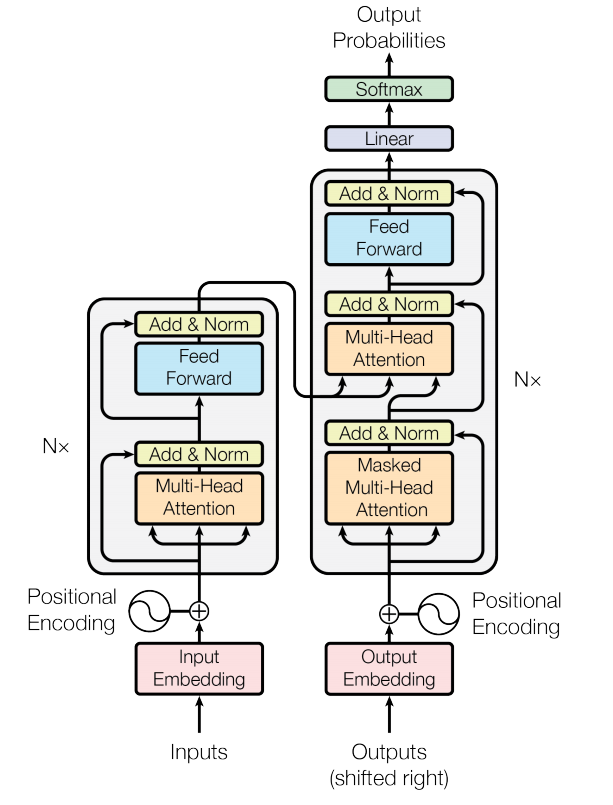
\includegraphics[width=1.0\textwidth]{figures/transformer.png}
		\end{figure}
	\end{column}
\end{columns}
\let\thefootnote\footnote{\href{https://arxiv.org/abs/1706.03762}{\color[rgb]{0.5,0.5,0.5} [Vaswani et al., 2017]}}
\end{frame}

\begin{frame}[c]{Attention is all you need}
\begin{columns}[c]
	\begin{column}{0.6\textwidth}
		\begin{itemize}
			\setbeamertemplate{itemize items}[square]
			\item Каждое слово параллельно проходит через слои кодировщика:
			\begin{itemize}
				\setbeamertemplate{itemize items}[circle]
				\item Каждый слой состоит из \textbf{multi-head attention} и полносвязной сети.
				\item Каждый подслой использует residual connections и layer normalization.
				\item Стекаем $N = 6$ таких слоев. 
			\end{itemize}
		\end{itemize}
	\end{column}
	\begin{column}{0.4\textwidth}
		\begin{figure}
			\centering
			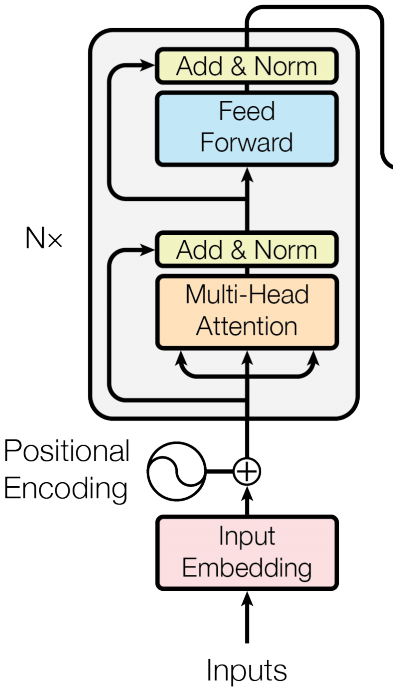
\includegraphics[width=0.8\textwidth]{figures/tranformer_encoder.png}
		\end{figure}
	\end{column}
\end{columns}
\end{frame}

\begin{frame}[c]{Attention is all you need}
\begin{columns}[c]
	\begin{column}{0.6\textwidth}
		\begin{itemize}
			\setbeamertemplate{itemize items}[square]
			\item Scaled dot-product attention: $Attention(Q,K,V)=softmax(\frac{QK^T}{\sqrt{n}})V$.
			\item $K$ и $V$ -- это всегда один и тот же вектор.
		\end{itemize}
	\end{column}
	\begin{column}{0.4\textwidth}
		\begin{figure}
			\centering
			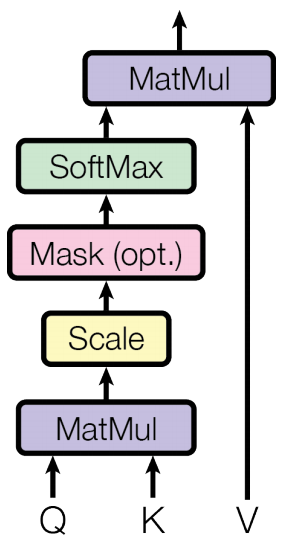
\includegraphics[width=0.6\textwidth]{figures/scaleddotattention.png}
		\end{figure}
	\end{column}
\end{columns}
\end{frame}

\begin{frame}[c]{Attention is all you need}
\begin{columns}[c]
	\begin{column}{0.7\textwidth}
		\begin{itemize}
			\setbeamertemplate{itemize items}[square]
			\item Multi-head attention: специальный новый слой, который дает возможность каждому входному вектору взаимодействовать с другими словами через attention mechanism.
			\item $MultiHead(Q,K,V) = [head_1, \cdots,head_h]W^O,$ где  $head_i=Attention(QW^Q_i,KW^K_i,VW^V_i)$
		\end{itemize}
	\end{column}
	\begin{column}{0.3\textwidth}
		\begin{figure}
			\centering
			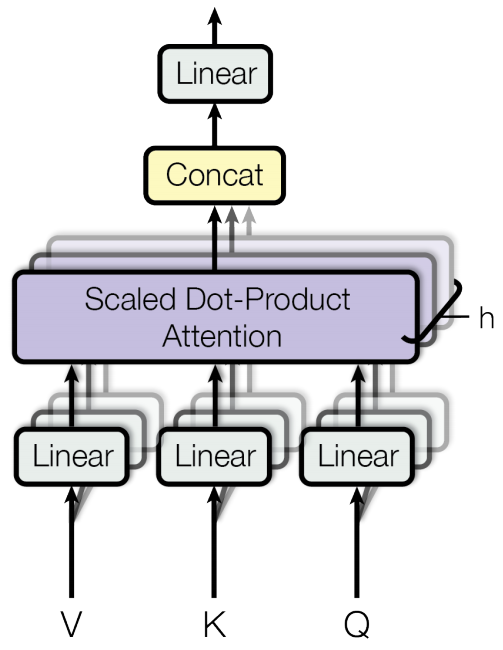
\includegraphics[width=1.0\textwidth]{figures/multiheadattention.png}
		\end{figure}
	\end{column}
\end{columns}
\end{frame}

\begin{frame}[c]{Attention is all you need}
\begin{columns}[c]
	\begin{column}{0.7\textwidth}
		\begin{itemize}
			\setbeamertemplate{itemize items}[square]
			\item Декодировщик запускается по слову за раз: получает на вход прошлое слово и должен выдать следующее.
			\item Два типа использования Multi-head attention:
			\begin{itemize}
				\setbeamertemplate{itemize items}[circle]
				\item Возможность обратиться к векторам прошлых декодированных слов.
				\item Возможность обратиться к выходу кодировщика.
			\end{itemize}
		\end{itemize}
	\end{column}
	\begin{column}{0.3\textwidth}
		\begin{figure}
			\centering
			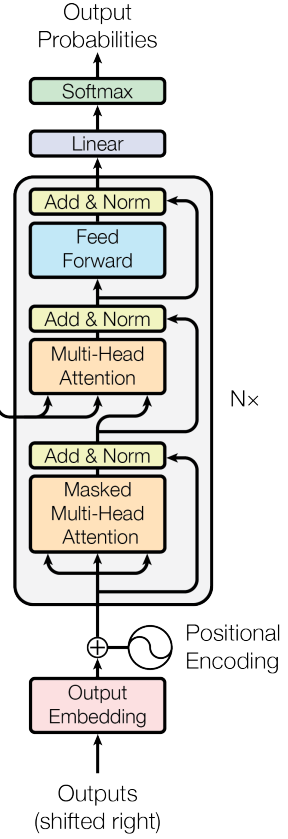
\includegraphics[width=0.7\textwidth]{figures/transformerdecoder.png}
		\end{figure}
	\end{column}
\end{columns}
\end{frame}

\begin{frame}[c]{Attention is all you need}
\begin{itemize}
	\setbeamertemplate{itemize items}[square]
	\item В итоге:
\end{itemize}
	\begin{figure}
		\centering
		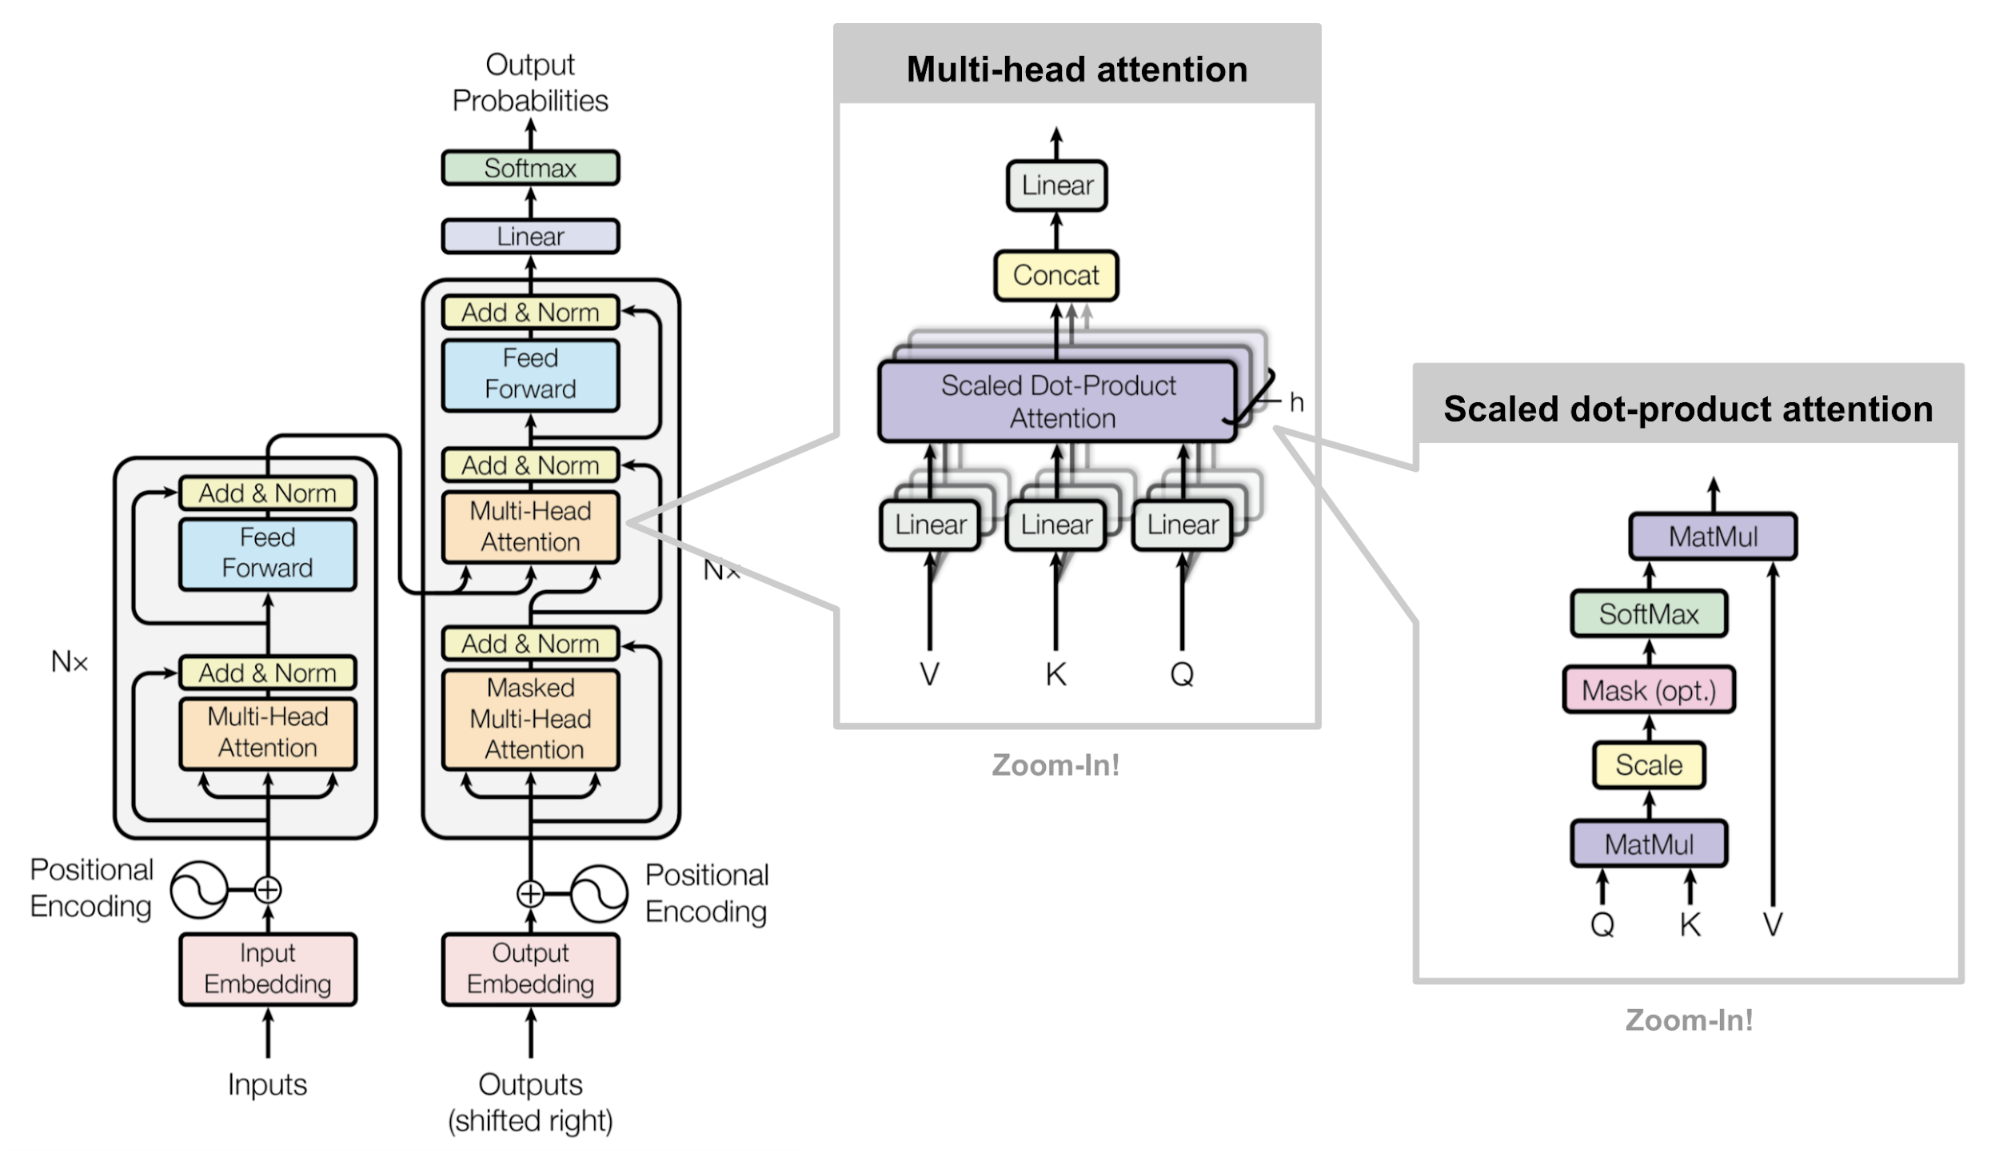
\includegraphics[width=1.0\textwidth]{figures/transformer_full.png}
	\end{figure}

\end{frame}


\begin{frame}[c]{Attention is all you need}
\begin{itemize}
	\setbeamertemplate{itemize items}[square]
	\item Результаты:
\end{itemize}
\begin{figure}
	\centering
	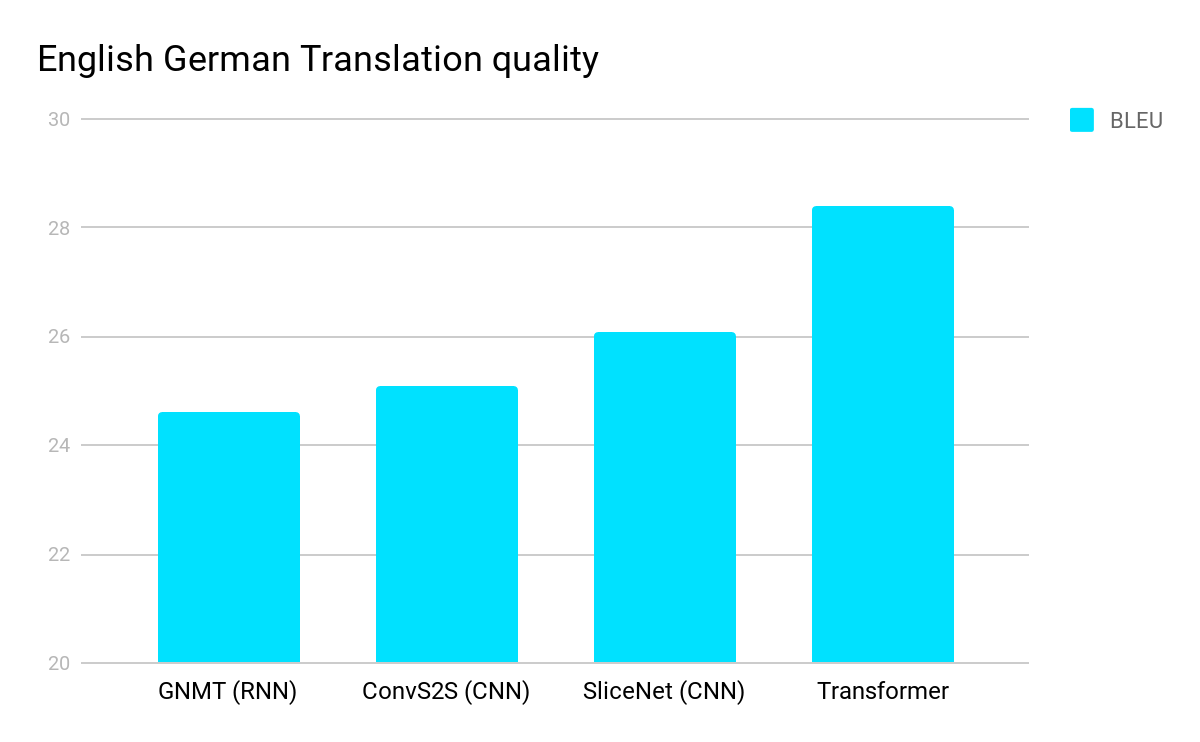
\includegraphics[width=0.8\textwidth]{figures/transformer_res.png}
\end{figure}
\end{frame}

\begin{frame}[c]{Attention is all you need}
\begin{itemize}
	\setbeamertemplate{itemize items}[square]
	\item Результаты:
\end{itemize}
\begin{figure}
	\centering
	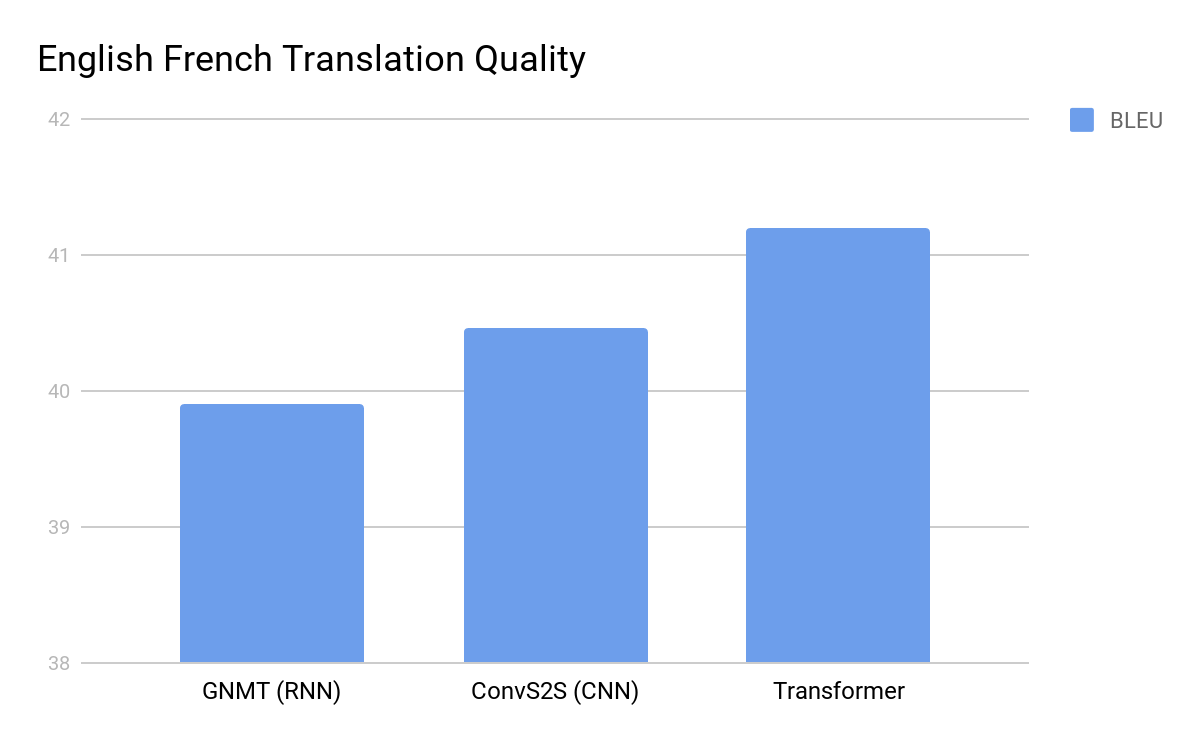
\includegraphics[width=0.8\textwidth]{figures/tranformer_res1.png}
\end{figure}
\end{frame}



